\chapter{Authentication II: \texttt{SSO} \& \texttt{SAML}}
\label{chap:authentication-ii}
\thispagestyle{chapterInit}
Questo capitolo è dedicato all'approfondimento dell'autenticazione all'interno di internet, in particolare verrà trattato il concetto di \texttt{Single Sign-On} per la riduzione del numero di credenziali da memorizzare e la gestione di queste ultime. Inoltre verrà trattato il protocollo \texttt{SAML} ovvero \textit{Security Assertion Markup Language} per la gestione di autenticazioni e autorizzazioni tra domini diversi, infine si parlerà di \texttt{SPID}, \texttt{CIE} \& \texttt{eIDAS} come esempi di implementazioni a livello nazionale ed europeo di \texttt{SSO}.
\section{Single Sign-On (\texttt{SSO})}
    \label{sec:sso}
    Il concetto alla base per il \texttt{SSO} è quello di avere un'unica autenticazione per accedere a (quasi) tutti i servizi, per raggiungere questo scopo il fornitore di servizi (\texttt{SP}) demanda il processo di autenticazione ad una autorità di identità (\texttt{IdP}) che si occupa di verificare che l'utente sia chi dice di essere, tramite i meccanismi visti precedentemente nella sezione \ref{sec:user-authentication}\footnote{\nameref{sec:user-authentication}}, mentre il processo di \textit{outsourcing} del processo di autenticazione è stato trattato nella sezione \ref{sec:outsourcing-authentication} \footnote{\nameref{sec:outsourcing-authentication}}.
    \paragraph{Funzionamento} Il funzionamento di un sistema \texttt{SSO} è il seguente:
        \begin{enumerate}
            \item L'utente accede all'applicazione \texttt{SP}
            \item L'applicazione \texttt{SP} reindirizza l'utente all'\texttt{IdP} per il processo di autenticazione
            \item L'\texttt{IdP} in primo luogo chiede all'utente di autenticarsi, il quale fornisce le proprie credenziali e l'\texttt{IdP} verifica l'identità dell'utente
            \item L'\texttt{IdP} genera un \textit{token} che viene cifrato e firmato con la chiave privata dell'\texttt{IdP} e inviato all'applicazione \texttt{SP}
            \item L'applicazione \texttt{SP} verifica la firma del \textit{token} con la chiave pubblica dell'\texttt{IdP} e se la verifica è positiva lo considera valido e lo inoltra all'utente che lo utilizzerà per accedere ai servizi (includendolo nelle richieste)
        \end{enumerate}
        Questo è il processo che avviene usualmente ma è possibile che il \textit{token} venga inviato all'utente dell'\texttt{IdP} e non direttamente all'applicazione del \texttt{SP}. In questo caso l'utente verifica la firma del \textit{token} con la chiave pubblica dell'\texttt{IdP} e poi lo includerà nelle richieste ai servizi.
    \paragraph{Proprietà} Le principali proprietà e vantaggi di un sistema \texttt{SSO} includono: la conservazioni delle credenziali in un unico posto e il non trasferimento delle stesse ad ogni servizio, i \textit{service provider} devono fidarsi dell'\textit{identity provider} nel verificare l'identità dell'utente. Inoltre il processo di autenticazione deve essere protetto, questo scopo lo si raggiunge usando la crittografia a chiave pubblica \footnote{ vedi \nameref{sec:PKI}} e con meccanismi di firma digitale.
    In questo paradigma è importante che l'\texttt{IdP} sia affidabile e che sia in grado di proteggere la \textit{confidentiality} e l'\textit{integrity} dei dati, inoltre è importante che l'\texttt{IdP} rimanga disponibile in quanto questo è un cosiddetto \textit{single point of failure}.
\section{Security Assertion Markup Language (\texttt{SAML})}
    \texttt{SAML} è un paradigma di autenticazione standard che sfrutta il formato \texttt{XML} per lo scambio di informazioni, questo lo rende molto \textit{verbose} anche per una piccola porzione di dati. Questo standard è stato introdotto nel 2002 e aggiornato nel 2005 in risposta alla mancanza di standard per lo scambio di informazioni di autenticazione e autorizzazione tra domini diversi.
    
    \paragraph{Esempio d'uso di \texttt{SAML}} In uno scenario dove ad esempio per avere uno sconto sul noleggio di un'auto è necessario essere membri VIP di una compagnia aerea, allora un utente (\textit{alice}) eseguirà il login sul sito della compagnia aerea (che agisce da \texttt{IdP} e \texttt{SP}) e poi verrà reindirizzata al sito di noleggio auto (che agisce solo da \texttt{SP}) con le informazioni dello status VIP dell'utente. A questo punto \textit{alice} può ottenere lo sconto da parte del sito di noleggio auto anche senza essersi autenticata su quest'ultimo, in quanto valgono le informazioni inviate dal sito della compagnia aerea.
    
    \begin{wrapfigure}{r}{0.2\textwidth}
        \centering
        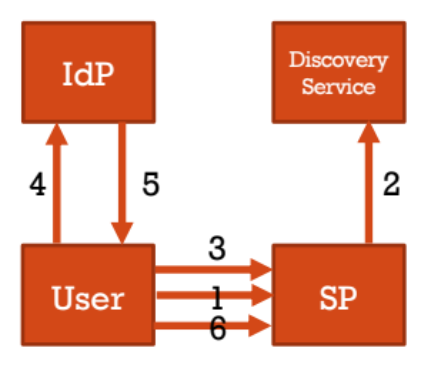
\includegraphics[width=0.2\textwidth]{05/SAML-Auth.png}
        \caption{Esempio di utilizzo di \texttt{SAML}}
    \end{wrapfigure}
    In breve:
        \begin{enumerate}
            \item L'utente vuole accedere ad un servizio \texttt{SP}
            \item Questo servizio \texttt{SP} reindirizza l'utente ad un \textit{Discovery Service} che permettere all'utente di scegliere l'\texttt{IdP} per l'autenticazione
            \item Dopo essersi registrato tramite il \texttt{IdP} scelto l'utente torna al servizio \texttt{SP} con una identità valida verificato da un \texttt{IdP}
            \item Allora il fornitore di servizi rimanda l'utente al suo \texttt{IdP} per ottenere un \textit{token} di autorizzazione
            \item L'utente si autentica sul \texttt{IdP} e ottiene un \textit{token} di autorizzazione
            \item L'utente ritorna al servizio \texttt{SP} con il \textit{token} di autorizzazione e può accedere ai servizi
        \end{enumerate}
    
    \subsection{\texttt{SAML} Overview}
        Come mostrato in figura \ref{fig:saml-overview} l'architettura di \texttt{SAML} è composto da diversi componenti quali:
        \begin{description}
            \item[\textit{Assertions}] - Le dichiarazioni fatte dal \texttt{IdP} riguardo l'identità dell'utente
            \item[\textit{Protocols}] - I protocolli usati per lo scambio di informazioni tra i vari componenti
            \item[\textit{Bindings}] - I meccanismi usati per associare i protocolli di \texttt{SAML} con i protocolli di comunicazione
            \item[\textit{Profiles}] - La combinazione di \textit{Assertions}, \textit{Protocols} e \textit{Bindings} a supporto di uno specifico caso d'uso
            \item[\textit{Authentication Context}] - Un dettaglio sui tipo di autenticazione e livello di sicurezza
            \item[\textit{Metadata}] - Dati di configurazione per \texttt{IdP} e \texttt{SP}
        \end{description}
        \begin{figure}[H]
            \label{fig:saml-overview}
            \centering
            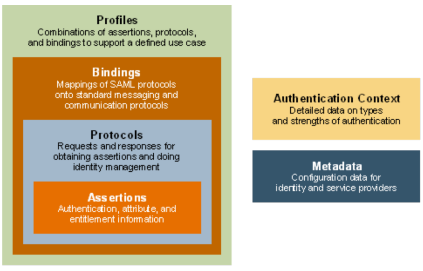
\includegraphics[width=0.5\textwidth]{05/SAML-Overview.png}
            \caption{Overview di \texttt{SAML}}
        \end{figure}
        \subsubsection{\textit{Assertions}}
            Le \textit{Assertions} sono le dichiarazioni fatte da una \texttt{SAML} \textit{authority} detta anche "parte dichiarante" (\textit{asserting party}). Le assertions possono essere viste come le unità di informazione di \texttt{SAML} e sono divise in tre tipi:
            \begin{description}
                \item[\textit{Authentication Assertion}] - Rilasciato dalla parte che autentica l'utente, contiene informazioni quali: chi ha autenticato l'utente, chi è il soggetto autenticato, quando è valida l'autenticazione, ecc\dots
                \item[\textit{Attribute Assertion}] - Contiene informazioni sullo stato dell'utente, come nell'esempio di \textit{alice} l'appartenenza al programma VIP
                \item[\textit{Authorization Assertion}] - Contiene informazioni su cosa può fare l'utente, come ad esempio la possibilità di noleggiare un'auto quando in viaggio di lavoro
            \end{description}
            \paragraph{\textit{Authentication Assertion}}
                Questo tipo di \textit{assertion} è strutturato nel seguente modo:
                \begin{description}
                    \item[Intestazione] - Contiene informazioni sulla versione di \texttt{SAML} usata, lo schema per \texttt{XML} e l'ora di creazione (\textit{issue instant})
                    \item[Autorità] - Contiene informazioni sul \texttt{IdP} che ha rilasciato l'\textit{assertion}
                    \item[Soggetto] - Contiene un identificativo univoco che rappresenta l'utente autenticato
                    \item[Condizioni] - Contiene informazioni sulla validità dell'\textit{assertion} (vale non prima di, non dopo il) con data e ora
                    \item[\textit{Authenticating Context}] - Contiene informazioni sul tipo di autenticazione e il livello di sicurezza che è stato usato\footnote{Si noti come la autenticazione in se non è parte del \texttt{SAML}, nelle \textit{assertion} ci si riferisce ad un processo di autenticazione avvenuto precedentemente}
                \end{description}
            \paragraph{\textit{Attribute Assertion}}
                Questo tipo di \textit{assertion} è strutturato nel seguente modo:
                \begin{description}
                    \item[Intestazione] - Contiene informazioni sulla versione di \texttt{SAML} usata, lo schema per \texttt{XML} e l'ora di creazione (\textit{issue instant}) l'unica differenza con l'\textit{Authentication Assertion} è il tipo di schema usato
                    \item[Attributo] - Contiene un identificatore del tipo di attributo (solitamente in modo molto specifico) e il valore dell'attributo
                \end{description}
        \subsubsection{\textit{Protocols}}
            I protocolli sono i meccanismi usati per lo scambio di asserzioni tra le varie parti e descrivono come poterne ottenerne una, come usarla e come verificarla. Vengono definiti anche protocolli sulle richieste di autenticazione e sulla risoluzione di parametri "passati per riferimento", viene definito anche un protocollo per il \textit{single logout} e per la gestione delle sessioni, e molo altro\dots\newline
            Distinguiamo come protocolli di comunicazione quei sistemi che permettono a due o più entità di scambiarsi informazioni definendo regole, semantica, sintassi e sincronizzazione. Esistono inoltre i protocolli di criptografia che sono designati alla protezione della comunicazione tra due entità, vengono applicati usando i \textit{cryptographic primitives} (come funzioni di \textit{hash}, cifrature simmetriche e asimmetriche, ecc\dots).
        \subsubsection{\textit{Bindings}}
            I \textit{bindings}, come anticipato, sono i meccanismi usati per definire i meccanismi per il trasporto dei messaggi \texttt{SAML} su protocolli di comunicazione diversi, come ad esempio \texttt{SAML URI}, \texttt{SAML SOAP}, \texttt{HTTP Redirect}, \texttt{HTTP POST}, ecc\dots
            \paragraph{\texttt{HTTP Redirect}} Questo meccanismo, in particolare, permette la trasmissioni di messaggi \texttt{SAML} tramite parametri di \texttt{URL} in una richiesta. In questo modo viene usato lo \textit{UserAgent} come intermediario per la trasmissione dei messaggi, questo meccanismo potrebbe essere necessario se è richiesta l'interazione con l'utente per generare una risposta. Questo è di gran lunga il meccanismo più usato (oltre che il preferito) per la trasmissione di messaggi \texttt{SAML} e per il \texttt{SSO}.
        \subsubsection{\textit{Profiles}}
            I \textit{profiles} sono le specifiche che definiscono come usare le \textit{assertions}, i \textit{protocols} e i \textit{bindings} per supportare uno specifico caso d'uso. Questi profili sono definiti per specifici scenari di utilizzo e sono usati per definire le regole di interazione tra le varie parti. I profili sono definiti per specifici scenari di utilizzo e sono usati per definire le regole di interazione tra le varie parti. 
            \paragraph{\textit{Web browser \texttt{SSO}}} Il profilo più comune è il \textit{web browser \texttt{SSO}} il quale ha più opzioni per quello che riguarda l'inizio e il trasporto dei messaggi \texttt{SAML}. L'inizio del flusso dei messaggio può essere inizializzato dal \texttt{SP} o dal \texttt{IdP} e il trasporto dei messaggi può essere eseguito tramite diversi \textit{bindings} quali \texttt{HTTP Redirect}, \texttt{HTTP POST}, \texttt{HTTP Artifact}, ecc\dots
            \paragraph{\textit{Single Logout}} Questo profilo è usato per terminare tutte le sessioni attive di un utente in una specifica rete \texttt{SAML}. In questo profilo l'utente ha stabilito un precedenza più sessioni con più \texttt{SP} ed un \texttt{IdP} e vuole terminare tutte le sessioni attive. Le sessioni gestite da una \textit{Session Authority} (\texttt{SeA}) che è un'entità che mantiene le informazioni sulle sessioni attive e che permette di terminarle (molto spesso è l'\texttt{IdP}). Quando l'utente vuole terminare la sessione, invia una richiesta di \textit{logout} alla \texttt{SeA} che termina tutte le sessioni attive inviando un messaggio di \textit{logout} a tutti i \texttt{SP} e all'\texttt{IdP}.
        \subsubsection{\textit{Authentication Context}}
            Questo componente indica come un utente si è autenticato presso un \texttt{IdP}. È quindi compito dell'\texttt{IdP} includerlo nelle \textit{assertions} in base alle richieste del \texttt{SP} o in base alla configurazione dell \texttt{IdP}. Le informazioni dentro l'\textit{authentication context} vengono usate per determinare il "livello di assicurazione" dell'autenticazione, ovvero quanto si è certi che l'utente sia chi dice di essere e di conseguenza quante e quali risorse può accedere. Solitamente un \textit{Level Of Assurance} (\texttt{LoA}) è costituito da un numero e definito in base al "valore" del "rischio" che è necessario per l'accesso alle risorse, questi livelli si basano principalmente su nozioni base di autenticazione.
        \subsubsection{\textit{Metadata}}
            Questo componente è usato per definire i dati di configurazione per \texttt{IdP} e \texttt{SP} e contiene informazioni quali: qual è l'identificativo dell'entità, le chiavi di criptografia, gli \textit{endpoints} per la comunicazione, ecc\dots Ogni entità di un sistema \texttt{SAML} ha un \textit{entity ID} che la identifica univocamente all'interno del sistema. Questo viene usato per associare le chiavi pubbliche alle entità e quindi per verificare le firme digitali. In entrambi le situazione gli \textit{id} e le chiavi pubbliche devono essere scambiate precedentemente in modo sicuro.
        
            
        \subsubsection{Correlazione tra le componenti}
            Le componenti di \texttt{SAML} sono correlate tra loro in questo modo: b
            \begin{description}
                \item[\textit{Assertions \& Protocols}] - Corrispondono al livello di applicazione del modello \texttt{ISO/OSI}. Da questo livello abbiamo la \textit{SSO experience}.
                \item[\textit{Bindings}] - Sono posizionati tra il livello dei profile e il livello applicazione.
                \item[\textit{Profiles}] - Sono posizionati al sotto il livello di applicazione e comunicano con questo tramite i \textit{bindings}.
            \end{description}
            I \textit{profiles} insieme ai \textit{bindings} costituiscono il \textit{web-service} dove sono specificate le tecnologie da usare quali \texttt{XML}, \texttt{URL}, \texttt{HTTP}, \texttt{HTTPS}, \texttt{SOAP}, ecc\dots
    \subsection{La sicurezza di \texttt{SAML}}
        La sicurezza di \texttt{SAML} non è propriamente intrinseca al protocollo, in quanto un semplice attacco del tipo \textit{men-in-the-middle} potrebbe ottenere la \textit{assertion} e usarla più tardi sostituendosi all'utente. Per questo motivo il protocollo \texttt{SAML} definisce, oltre ai meccanismi di scambio di informazioni, anche i meccanismi di protezione delle informazioni scambiate, principalmente viene usata la \texttt{PKI}\footnote{Vedi \ref{sec:PKI} \nameref{sec:PKI}} la quale però non è obbligatoria, ma è fortemente raccomandata.
        \paragraph{Qualche possibile attacco} Alcune possibili vulnerabilità di \texttt{SAML} riguardano: il tempo di validità di un \textit{assertion}, risolvibile inserendo una durata relativamente breve, la ripetizione di un \textit{assertion}, risolvibile inserendo accettando solo una volta un \textit{assertion} con uno stesso \texttt{ID}, la ricezione di un \textit{assertion} per un \textit{SP} diverso, tutti i \textit{SP} devono accettare solo ed esclusivamente i messaggi destinati a loro e non a un altro \textit{SP}. Inoltre esiste una possibile vulnerabilità relativa a \texttt{XXE} o \textit{XML External Entity}, il quale sfrutta il fatto che \texttt{SAML} è basato su \texttt{XML} inviati dall'utente e poi processati dal \texttt{SP}, ma in quanto \texttt{XML} è molto pesante da processare ciò potrebbe portare ad un \textit{DoS} o ad un \textit{XXE}.

        \paragraph{Privacy e \texttt{SAML}} La privacy è un aspetto molto importante per \texttt{SAML} in quanto le informazioni scambiate sono molto sensibili, allora è possibile non scambiare direttamente le informazioni ma passare solo un codice identificativo dell'entità che possa essere usato per recuperare le informazioni dal \texttt{IdP}. Il problema però rimane che se l'\texttt{IdP} è compromesso o "venduto" allora tutte le informazioni, sia quelle di tipo identificativo che quelle associate ad un "\textit{log}" dei servizi a cui si è acceduto, sono a rischio.
\section{Infrastruttura di identità nazionale}
    \subsection{\texttt{SPID} - Sistema Pubblico di Identità Digitale}
        \paragraph{Struttura generale} Lo \texttt{SPID} è un sistema di identità digitale che permette di accedere a tutti i servizi online della pubblica amministrazione e di altri enti privati con un'unica identità digitale. Questo sistema si basa su \texttt{SAML 2.0} ma esistono due entità in più, la prima è "\texttt{AgID}" che ha il compito di coordinare e gestire il sistema fornendo ai \texttt{SP} l'elenco degli \texttt{IdP} autorizzati e la seconda è \textit{Attribute Provider} che fornisce informazioni aggiuntive sull'utente. A linee generali il funzionamento è lo stesso di \texttt{SAML} con l'aggiunta di un "passo 0" che consiste nel \texttt{SP} che chiede ad \texttt{AgID} l'elenco degli \texttt{IdP} autorizzati e un passaggio opzionale per il \texttt{SP} che chiede all'\textit{Attribute Provider} informazioni aggiuntive sull'utente.
        \paragraph{La legge} A livello legale per diventare \texttt{IdP} o \texttt{SP} bisogna rispettare delle norme sia a livello italiano che a livello europeo, queste norme si pongono al di sopra dello standard \texttt{SAML} e all'infrastruttura tecnica, queste sono state introdotte per aumentare il livello di sicurezza e di privacy delle informazioni scambiate, inoltre prevedono che se necessario a livello giudiziario si possano ottenere (parte) delle informazioni scambiate. 
    \subsection{\texttt{CIE 3.0} - Carta d'Identità Elettronica}
        La carta di identità elettronica usa lo stesso protocollo usato da \texttt{SPID}, ma in quanto l'autenticazione non fà parte di \texttt{SAML} questa viene fatta in maniera diversa.
        \paragraph{Informazioni Contenute} La \texttt{CIE} contiene diverse informazioni personali come: nome, cognome, data e luogo di nascita, residenza, foto personale e due impronte digitali, le quali possono essere verificate solo dalle forze dell'ordine.
            \subparagraph{Validità} In modo da garantire l'aggiornamento delle informazioni contenute nella \texttt{CIE} questa ha una validità variabile in base all'età del titolare: 3 anni per i minori di 3 anni, 5 anni per i minori di 18 anni e 10 anni per gli adulti.
        \paragraph{Capacità} La \texttt{CIE} usa la tecnologia \texttt{NFC}, usata per la comunicazione a corto raggio ($\leq 4cm$) con una bassa velocità.\footnote{la tecnologia \texttt{NFC} viene usata anche per pagamenti \textit{contactless}} Questa tecnologia permette di leggere le informazioni contenute nella \texttt{CIE} e di autenticare l'utente, inoltre la \texttt{CIE} può essere usata per la firma digitale.
            \subparagraph{Criptografia} All'interno della \texttt{CIE} sono presenti diversi \textit{chips} contenenti meccanismi di crittografia per la protezione delle informazioni. Vengono usati all'interno della \texttt{CIE} i protocolli \texttt{AES} (256 bits) e \texttt{3DES} (112 bits), \texttt{SHA-2} e \texttt{SHA-1}, \textit{Diffie-Hellman} a 2048 bits e \texttt{RSA (v1.5)} a 2048 bits. \texttt{X.509} è usato per la firma digitale e per la verifica delle firme.\newline
        Di queste non tutte le combinazioni sono possibili. 
        \subsubsection{Funzionamento}
            \paragraph{Registrazione \texttt{CIE Id}} In primo luogo bisogna registrare la propria \texttt{CIE} tramite la applicazione: \texttt{CIE Id}, la quale, previo inserimento di pin per lo sblocco, permette di leggere le informazioni contenute nella \texttt{CIE} e di autenticare l'utente. Il pin nel processo di registrazione viene usato per "garantire alla \texttt{CIE} che l'utente è il legittimo proprietario della carta". 
            \paragraph{Accesso} Per eseguire l'accesso ad un servizio tramite la \texttt{CIE}: in primo luogo il \texttt{SP} deve mostrare il pulsante "Entra con \texttt{CIE}", poi viene chiesto l'inserimento del numero di serie della \texttt{CIE} per la generazione della \textit{challenge}, successivamente viene chiesto di inquadrare un \textit{QR code} con il proprio telefono sul quale è installata l'applicazione \texttt{CIE Id}, infine viene chiesto di inserire il pin e appoggiare la \texttt{CIE} al telefono per completare l'autenticazione.
            
        \paragraph{Sicurezza} Da notare come le informazioni su chi sia l'utente assieme a quelle per l'autenticazione sono conservate all'interno della \texttt{CIE}, in questo modo il server centrare non ha bisogno di memorizzare le informazioni dell'utente e quindi anche in caso di \textit{data breach} le informazioni di autenticazione e dell'utente sono al sicuro.

        Di seguito vengono riportati lo schema delle comunicazioni che avvengono tra le varie entità coinvolte nel processo di autenticazione con la \texttt{CIE} e il diagramma di sequenza per l'autenticazione con la \texttt{CIE}.
        \newpage
        
        \begin{figure}[H]
            \centering
            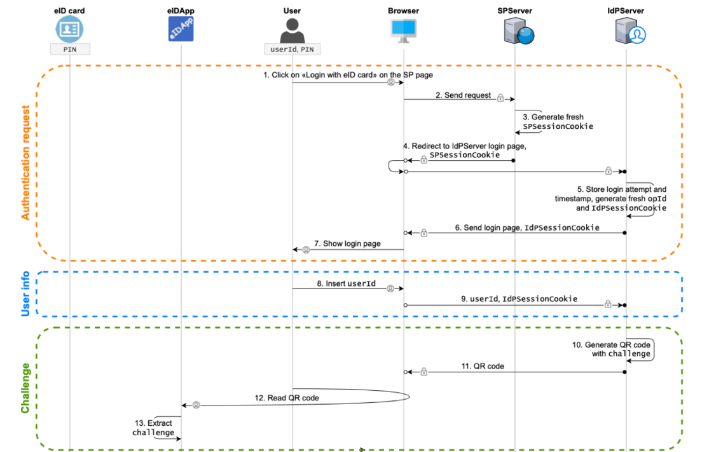
\includegraphics[width=0.45\textwidth]{05/CIE-auth-01.png}
            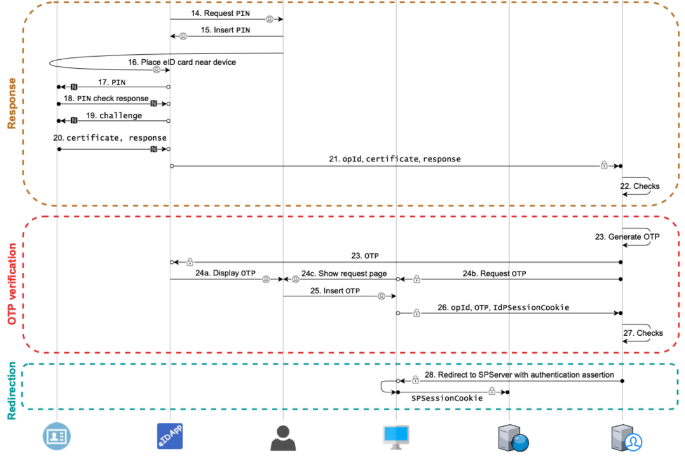
\includegraphics[width=0.45\textwidth]{05/CIE-auth-02.png}
            \caption{Diagramma di sequenza per l'autenticazione con la \texttt{CIE} - Parte 1}
        \end{figure}

        Di questi l'importante è notare la quantità di attori coinvolti: "\texttt{CIE}", "\texttt{CIE Id} App", "Utente", "\textit{Browser}", "\texttt{SP} \textit{server}" e "\texttt{CIE Id} \textit{server}". Questo è un esempio di un sistema di autenticazione molto complesso, ma decentralizzato e sicuro, in questo caso a differenza dello \texttt{SPID} non c'è un \textit{single point of failure}. Notare inoltre le diverse fasi: "\textit{Authentication request}", "\textit{User Info}", "\textit{Challenge}", "\textit{Response}", "\textit{OTP verification}" e "\textit{Redirection}".
        \subsubsection{Livello di sicurezza} 
            Inizialmente il livello di sicurezza di \texttt{CIE} è stato paragonato ad una autenticazione \texttt{SPID} di livello 3, successivamente in quanto è sorta la necessità di creare dei livelli 1 e 2 per l'autenticazione ad alcuni servizi online si è deciso di creare un \textit{server} centralizzato per l'autenticazione tramite \textit{username} e \textit{password}, di fatto portando il livello di sicurezza della \texttt{CIE} molto più simile ad una autenticazione \texttt{SPID}. Quindi ora è possibile autenticarsi con la \texttt{CIE} a livello 1, 2 e 3 come per lo \texttt{SPID}.
    \subsection{\texttt{eIDAS} - \textit{European Identity Infrastructure}}
        \paragraph{Struttura generale} Questo sistema è nato per usare un'unica identità digitale per accedere a tutti i servizi europei, questo senza il bisogno di "creare" una nuova identità digitale per il paese in cui si vuole accedere. Il sistema si pone sopra al livello dello \texttt{SPID} o altri sistemi di identità nazionali e tramite dei "nodi" e "\textit{connector}" permette la comunicazione tra i vari sistemi nazionali. 
        \paragraph{Esempio d'uso e funzionamento} Ponendo che un cittadino con identità digitale italiana voglia accedere ad un servizio in germania, in questo caso il \textit{eIDAS-Connector} tedesco inizializza una connessione diretta con il \texttt{SP} e invia una richiesta al \textit{eIDAS-Service} italiano, ora il \textit{eIDAS-Service} italiano chiede all'utente quale \texttt{IdP} si intende utilizzare e si procede con l'autenticazione. Una volta ottenuta l'autenticazione l'\textit{eIDAS-Service} italiano risponde alla richiesta del \textit{eIDAS-Connector} tedesco con le informazioni necessarie per l'accesso al servizio.
        \subsubsection{Vulnerabilità}
            Questo sistema si basa sulla sicurezza dell'autenticazione di ogni stato membro e dei suoi \textit{connector}, è dunque indispensabile che ogni stato sia allineato con le normative europee e che i \textit{connector} siano sicuri. Inoltre in quanto avviene uno scambio diretto di messaggi tra \textit{connector} il canale di comunicazione deve essere sicuro e protetto, altrimenti un attaccante potrebbe inviare come risposta al \textit{connector} del paese di destinazione un messaggio fasullo e ottenere l'accesso ai servizi altrui.
            \paragraph{Certificati non firmati} Nel 2019 è avvenuto un attacco a \texttt{eIDAS} che ha sfruttato il fatto che durante il processo di autenticazione il nodo ricevente non controllava che il certificato fosse correttamente firmato da una autorità di certificazione fidata, i messaggi erano firmati ma non da una autorità fidata, venivano infatti accettati certificati che sembrano firmati da una autorità fidata ma che in realtà non lo erano (parametri di sicurezza non corretti)
        \subsubsection{\texttt{eIDAS 2.0}}
            \paragraph{Obiettivi} Questa nuova versione di \texttt{eIDAS} ha come obiettivo quello di creare un "portafoglio digitale" per tutti i cittadini europei, in modo da poter conservare tutti i propri documenti (anche di identità) in un unico posto e poterli usare a valore legale in tutti i paesi europei. Oltre ai documenti di identità quali la carta d'identità elettronica, la patente di guida, ecc\dots si potranno conservare anche i diplomi universitari, le certificazioni di lavoro, ecc\dots
            \paragraph{Funzionamento Base} Di base \texttt{eIDAS 2.0} prevede una decentralizzazione delle identità, conservate sui dispositivi degli utenti, e una centralizzazione dei soli \textit{hash} per la verifica che le informazioni effettivamente contenute nel \textit{wallet} siano quelle corrette. Il sistema rimane sicuro in quanto le informazioni conservate in un \textit{wallet} sono prima rilasciate da un \textit{issuer} che può essere il ministero, l'università, ecc\dots, vengono successivamente conservate nel \textit{wallet} e l'\textit{hash} viene inviato alla \textit{ESSIF Blockchain} per la verifica futura. Quando un utente vuole presentare un documento, invia le informazioni di questo ad un \textit{Verifier} o \texttt{SP} che esegue le operazioni di \textit{hash} e verifica se nella \textit{ESSIF Blockchain} esiste un \textit{hash} corrispondente, se esiste allora il documento è valido.